%\documentclass{clases}
\documentclass[a4paper,12pt, oneside]{book}
\LoadClass[a4paper,12pt, oneside]{book}
\usepackage[skins,minted]{tcolorbox}
\usepackage[utf8]{inputenc}
\usepackage[T1]{fontenc}
\usepackage[spanish]{babel}
\languageshorthands{spanish}
\usepackage[numbers]{natbib}
%\usepackage{morewrites}
\usepackage{inconsolata}
\usepackage{mdframed}
\usepackage{minted}
\usepackage{listings}
\usepackage{subcaption}
\usepackage{amsmath}
\usepackage{amssymb}
\usepackage{graphicx, import}
\usepackage{hyperref}
\usepackage{longtable}
\usepackage{xcolor}
\usepackage{pdfpages}
%\usepackage{color}
\usepackage{fancyhdr}
\usepackage{menukeys}
\usepackage{appendix}
\usepackage{fontawesome}
\usepackage{comment}
\usepackage{caption}
\usepackage{setspace}
\usepackage[explicit]{titlesec}
\usepackage[a4paper]{geometry}
\geometry{top=3cm, bottom=3cm, left=4cm, right=2cm}
%\usepackage[draft]{listofsymbols}
%\usepackage[toc,acronym]{glossaries}
%\makeglossaries
%\glossarystyle{altlistgroup}

% se incluye el archivo de definición de acrónimos
%\include{acronimos}

% se incluye el archivo de definición de glsario
%\include{glosario}

%\opensymdef
%\input{capitulos/A2_simbolos}
%\closesymdef

\definecolor{green1}{HTML}{1dae28}
\definecolor{green2}{HTML}{afd095}
\definecolor{lightgray}{gray}{0.9}
\definecolor{orange}{RGB}{18,84,183}
\definecolor{titulo}{gray}{0.75}
\definecolor{gray97}{gray}{.97}
\definecolor{gray75}{gray}{.75}
\definecolor{gray45}{gray}{.45}
\definecolor{advertencia}{RGB}{255,178,102}
\definecolor{colorturqueza}{RGB}{178,223,238}
\definecolor{mintedbackground}{rgb}{0.95,0.95,0.95}
\definecolor{lbcolor}{rgb}{0.95,0.95,0.95}
\definecolor{mintedframe}{rgb}{0.0,0.0,0.0}
\lstset{
	frame=Ltb,
	tabsize=2,
	framerule=0pt,
	aboveskip=0.5cm,
	framextopmargin=0pt,
	framexbottommargin=0pt,
	framexleftmargin=0.4cm,
	framesep=0pt,
	rulesep=.0pt,
	backgroundcolor=\color{gray97},
	rulesepcolor=\color{blue},
	%
	stringstyle=\ttfamily,
	showstringspaces = false,
	basicstyle=\small\ttfamily,
	commentstyle=\color{gray45},
	keywordstyle=\bfseries,
	%
	numbers=none,
	numbersep=15pt,
	numberstyle=\tiny,
	numberfirstline = false,
	breaklines=true
}

\setminted[bash]{
	bgcolor=mintedbackground,
	fontfamily=tt,
	linenos=true,
	numberblanklines=true,
	numbersep=11pt,
	numbersep=2pt,
	gobble=0,
	frame=leftline,
	framesep=2mm,
	funcnamehighlighting=false,
	tabsize=4,
	obeytabs=false,
	samepage=false,
	showspaces=false,
	showtabs =false,
	texcl=false,
	baselinestretch=1.2,
	fontsize=\footnotesize,
	breaklines=true,
	breaksymbolleft=\ 
}


% minimizar fragmentado de listados
%\lstnewenvironment{listing}[1][]{\lstset{#1}\pagebreak[0]}{\pagebreak[0]}


\lstdefinestyle{consola}{
	basicstyle=\footnotesize\bf\ttfamily,
	backgroundcolor=\color{gray75},
}	
\definecolor{gray}{rgb}{0.4,0.4,0.4}
\definecolor{darkblue}{rgb}{0.0,0.0,0.6}
\definecolor{cyan}{rgb}{0.0,0.6,0.6}
\lstset{language=XML}

\lstdefinelanguage{XML}{
	morestring=[b]",
	tabsize=2,
	breaklines=true,
	morestring=[s]{>}{<},
	morecomment=[s]{<?}{?>},
	stringstyle=\color{black},
	identifierstyle=\color{darkblue},
	keywordstyle=\color{cyan},
	numbers=left,
	morekeywords={xmlns,version,type}% list your attributes here
}

\lstdefinestyle{C}{language=C}
\lstdefinestyle{XML}{language=XML}
\definecolor{codebg}{rgb}{0.96,0.96,0.96}
\definecolor{colorurls}{RGB}{107,17,17}
\definecolor{colorsql}{RGB}{255,245,245}
\definecolor{colorreferences}{RGB}{48,134,3}
\definecolor{titulo}{gray}{0.65}			%------ color para fondo del titulo de tablas.
\hypersetup{
	%bookmarks=true,         % show bookmarks bar?
	unicode=false,          % non-Latin characters in Acrobat’s bookmarks
	pdftoolbar=true,        % show Acrobat’s toolbar?
	pdfmenubar=true,        % show Acrobat’s menu?
	pdffitwindow=false,     % window fit to page when opened
	pdfstartview={FitH},    % fits the width of the page to the window
	pdftitle={Diseño de modelo para simulación 3D de VANT tipo cuadricóptero},    % title
	pdfauthor={Jesús Iván Medina Gil Lamadrid},     % author
	pdfsubject={Reporte final de residencias},   % subject of the document
	%pdfcreator={pdfTeX 3.14159265-2.6-1.40.16 (TeX Live 2016/dev)},   % creator of the document
	%pdfproducer={Panel HJ 2017}, % producer of the document
	pdfkeywords={simulación} {quadrotor} {vant} {ros} {gazebo} {hector\_quadrotor}, % list of keywords
	%pdfnewwindow=true,      % links in new PDF window
	colorlinks=true,       % false: boxed links; true: colored links
	linkcolor=black,          % color of internal links (change box color with linkbordercolor)
	citecolor=colorreferences,        % color of links to bibliography
	filecolor=magenta,      % color of file links
	urlcolor=blue,           % color of external links
	linkbordercolor={0 0 0}
}

\lstset{literate=
	{á}{{\'a}}1 {é}{{\'e}}1 {í}{{\'i}}1 {ó}{{\'o}}1 {ú}{{\'u}}1
	{Á}{{\'A}}1 {É}{{\'E}}1 {Í}{{\'I}}1 {Ó}{{\'O}}1 {Ú}{{\'U}}1
	{à}{{\`a}}1 {è}{{\`e}}1 {ì}{{\`i}}1 {ò}{{\`o}}1 {ù}{{\`u}}1
	{À}{{\`A}}1 {È}{{\'E}}1 {Ì}{{\`I}}1 {Ò}{{\`O}}1 {Ù}{{\`U}}1
	{ä}{{\"a}}1 {ë}{{\"e}}1 {ï}{{\"i}}1 {ö}{{\"o}}1 {ü}{{\"u}}1
	{Ä}{{\"A}}1 {Ë}{{\"E}}1 {Ï}{{\"I}}1 {Ö}{{\"O}}1 {Ü}{{\"U}}1
	{â}{{\^a}}1 {ê}{{\^e}}1 {î}{{\^i}}1 {ô}{{\^o}}1 {û}{{\^u}}1
	{Â}{{\^A}}1 {Ê}{{\^E}}1 {Î}{{\^I}}1 {Ô}{{\^O}}1 {Û}{{\^U}}1
	{œ}{{\oe}}1 {Œ}{{\OE}}1 {æ}{{\ae}}1 {Æ}{{\AE}}1 {ß}{{\ss}}1
	{ç}{{\c c}}1 {Ç}{{\c C}}1 {ø}{{\o}}1 {å}{{\r a}}1 {Å}{{\r A}}1
	{€}{{\EUR}}1 {£}{{\pounds}}1 {'}{{\textquotesingle}}1 {Ñ}{{\~N}}1
	{ñ}{{\~n}}1
}

\newtcblisting{terminal}[2][]{
	listing engine=minted,
	listing only,
	#1,
	title=#2,
	minted language=bash,
	colback=mintedbackground,
	top=0mm,
	bottom=0mm
}

\newtcblisting{consolestyle}[2][]{enhanced, listing engine=minted, 
	listing only,#1, title=#2, minted language=bash, 
	coltitle=mintedbackground!35!black, 
	fonttitle=\ttfamily\footnotesize,
	sharp corners, top=0mm, bottom=0mm,
	title code={\path[draw=mintedframe, dashed, fill=mintedbackground](title.south west)--(title.south east);},
	frame code={\path[draw=mintedframe, fill=mintedbackground](frame.south west) rectangle (frame.north east);}
}
\newenvironment{doble}
{\doublespacing
}

%\newcounter{comando}[section]
%\newenvironment{comando}[1][]{\refstepcounter{comando}\par\medskip
%	\noindent \textbf{Comando~\thecomando. #1} \rmfamily}{\medskip}
%\begin{terminal}{#1}
	
%\end{terminal}
%}{\medskip}

\graphicspath{ {img/} }

\begin{document}
	% Aquí se encuentra el archivo con la portada
	\begin{titlepage}
	\centering
	%-------------------------------------------
	% Logos en una tabla: izquierda, centro y derecha
	\begin{tabular}{@{}p{0.3\textwidth} p{0.3\textwidth} p{0.3\textwidth}@{}}
		
\includegraphics[height=2cm]{tecnm} & 
		\centering 
\includegraphics[height=1.5cm]{SEP} & 
		\raggedleft 
\includegraphics[height=2cm]{ith.jpg} \\
	\end{tabular}
	
	\vspace{2em}
	
	\noindent
	%-------------------------------------------
	%	Información institucional y académica (esquina superior izquierda)
	\begin{minipage}[t]{0.6\textwidth}
		\raggedright
		\small \textbf{%
			Instituto Tecnológico de Hermosillo\\
			Materia: Robótica\\
			Profesor: Medina Gil Lamadrid, Jesús Iván%
		}
	\end{minipage}%
	\hfill
	%	fecha actual (esquina superior derecha), en letras pequeñas y en negrita.
	\begin{minipage}[t]{0.3\textwidth}
		\raggedleft
		\small \textbf{\today}
	\end{minipage}
	
	\vspace{2em}
	
	%-----------------------------------------
	% Unidad y Título de la tarea en letras grandes y en negrita
%	{\large \textbf{Unidad Final}}\\
	{\Huge \textbf{Reporte final del Robot}}
		
	\vspace{1em}
	
	%---------------------------------------
	% Tabla con la información del equipo
	%---------------------------------------
	% Encabezado del equipo
	\begin{center}
		{\Large \textbf{Equipo 5}}
		
		{\small \textbf{https://github.com/JesusLazar/Robotica.git}}
	\end{center}
	
	\vspace{1em}
	
	% Tabla de integrantes:
	% Cada fila contiene: foto (columna izquierda) y datos del integrante (columna derecha)
	\begin{center}
		\begin{tabular}{c c}
			\begin{tabular}{c}
			
\includegraphics[height=3cm]{Mich.jpg} \\
				\textbf{Arvizu, }\\ Michelle \\ \texttt{l21330532@hermosillo.tecnm.mx } \\ Teléfono: (6221164719)
			\end{tabular} &
			\begin{tabular}{c}
				
\includegraphics[height=3cm]{Lazaro.jpg} \\
				\textbf{Carranza,}\\ Jesús \\ \texttt{l21330548@hermosillo.tecnm.mx} \\ Teléfono: (6621130410)
			\end{tabular} \\ \vspace{2em}
			\begin{tabular}{c}
				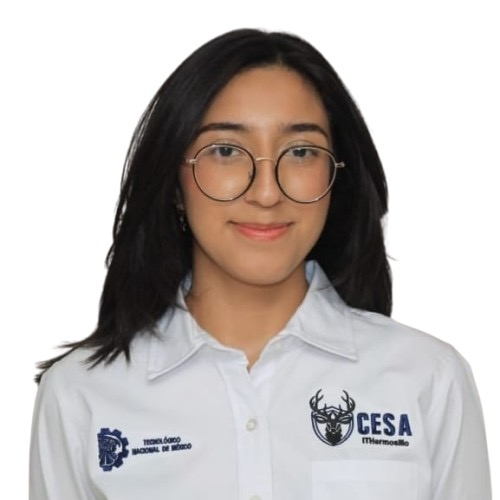
\includegraphics[height=3cm]{Morelia.jpg} \\
				\textbf{Montoya,}\\ Morelia \\ \texttt{l21330642@hermosillo.tecnm.mx} \\ Teléfono: (6624251581)
			\end{tabular} &
			\begin{tabular}{c}
				\includegraphics[height=3cm]{Anitafoto.jpg} \\
				\textbf{Moreno,}\\ Ana \\ \texttt{l21330650@hermosillo.tecnm.mx} \\ Teléfono: (6624591969)
			\end{tabular}
		\end{tabular}
	\end{center}

\end{titlepage}

	\onehalfspacing
	\frontmatter
	\pagestyle{plain}  % numeración en páginas preliminares
	\titleformat{\chapter}
	{\bfseries\huge}
	{}
	{0pt}
	{~\raisebox{-1.5pt}{}
	\\\filleft #1 \\\vspace{.25cm}\titlerule[1.5pt]}
	
	% ---------------------------------------
	% índices
%	\clearpage   % o \cleardoublepage, según prefieras
	\newpage
	\phantomsection    % crea un nuevo destino para hyperref
	\addcontentsline{toc}{chapter}{Índice general}
	\tableofcontents
	
%	\clearpage
	\newpage
	\phantomsection
	\addcontentsline{toc}{chapter}{Índice de figuras}
	\listoffigures
	
	\hypersetup{
		linkcolor=red
	}
	
	% ---------------------------------------
	% Estilo de encabezado y pie de página
	\mainmatter
	\pagestyle{fancy}
	\fancyhead{}
	\fancyhead[L]{\leftmark}
	\fancyhead[R]{}
	\fancyfoot[L]{\parbox[l]{\textwidth-1cm}{\rightmark}}
	\fancyfoot[C]{}
	\fancyfoot[R]{\thepage}
	\renewcommand{\footrulewidth}{0.5pt}
	%\fancyfoot[RO,LE]{Diseño de modelo para simulación 3D de VANT tipo cuadricóptero}
	
	\titleformat{\chapter}
	{\bfseries\huge}
	{}
	{0pt}
	{\titlerule[3pt]~\raisebox{-1.5pt}{\sc{\chaptername}~\thechapter}~\titlerule[3pt]%
		\\\vspace{.05cm}\titlerule\\\filcenter #1 \\\vspace{.25cm}\titlerule}
	
	% Capítulo 1: Introducción
	\chapter{Introducción} \label{chap:introduccion}

El presente trabajo tiene como objetivo documentar y analizar el desarrollo de un proyecto robótico realizado durante el semestre, el cual integra los principales conceptos estudiados en la asignatura de Robótica. Para este proyecto, se seleccionó un modelo de robot descargado directamente desde una plataforma en línea, el cual ya contaba con un diseño de ensamblado estructural completo. Esta elección permitió enfocar el trabajo en el análisis cinemático y en la aplicación de modelos matemáticos y conceptuales clave.

Una vez definido el modelo, se procedió a identificar sus ejes de rotación y sus coordenadas espaciales, lo que permitió establecer los parámetros necesarios para construir las tablas de Denavit-Hartenberg. A partir de estas tablas, se desarrolló la cinemática directa del robot, permitiendo determinar la posición y orientación del efector final en función de las variables articulares. Posteriormente, se abordó la cinemática diferencial, lo cual facilitó el análisis de velocidades y permitió una mejor comprensión del comportamiento dinámico del sistema.

Además, se resolvió el problema de la cinemática inversa, fundamental para el control del robot en tareas específicas, ya que permite calcular los valores articulares necesarios para alcanzar una determinada posición en el espacio. Todos estos análisis y cálculos se realizaron en concordancia con los contenidos abordados a lo largo del semestre, consolidando así los conocimientos teóricos mediante su aplicación práctica.

Este informe detalla cada una de estas etapas, presentando los fundamentos teóricos, los métodos aplicados y los resultados obtenidos, con el fin de demostrar el dominio adquirido en el manejo de herramientas y conceptos fundamentales en el campo de la robótica.
	
	% Capítulo 2: Marco Teórico
	\chapter{Introducción} \label{chap:introduccion}

El presente trabajo tiene como objetivo documentar y analizar el desarrollo de un proyecto robótico realizado durante el semestre, el cual integra los principales conceptos estudiados en la asignatura de Robótica. Para este proyecto, se seleccionó un modelo de robot descargado directamente desde una plataforma en línea, el cual ya contaba con un diseño de ensamblado estructural completo. Esta elección permitió enfocar el trabajo en el análisis cinemático y en la aplicación de modelos matemáticos y conceptuales clave.

Una vez definido el modelo, se procedió a identificar sus ejes de rotación y sus coordenadas espaciales, lo que permitió establecer los parámetros necesarios para construir las tablas de Denavit-Hartenberg. A partir de estas tablas, se desarrolló la cinemática directa del robot, permitiendo determinar la posición y orientación del efector final en función de las variables articulares. Posteriormente, se abordó la cinemática diferencial, lo cual facilitó el análisis de velocidades y permitió una mejor comprensión del comportamiento dinámico del sistema.

Además, se resolvió el problema de la cinemática inversa, fundamental para el control del robot en tareas específicas, ya que permite calcular los valores articulares necesarios para alcanzar una determinada posición en el espacio. Todos estos análisis y cálculos se realizaron en concordancia con los contenidos abordados a lo largo del semestre, consolidando así los conocimientos teóricos mediante su aplicación práctica.

Este informe detalla cada una de estas etapas, presentando los fundamentos teóricos, los métodos aplicados y los resultados obtenidos, con el fin de demostrar el dominio adquirido en el manejo de herramientas y conceptos fundamentales en el campo de la robótica.
	
		\section{Cinemática} \label{sec:cinematica}

La cinematica es una parte de la fisica que estudia el movimiento de los sistemas mecanicos sin tomar en cuenta las fuerzas que originan dicho movimiento. Se centra en la relacion geometrica entre las articulaciones del robot y su extremo efector, de esta forma permite predecir la posicion y orientacion en funcion de las posiciones articulares, y viceversa. Comprender la cinematica es vital para entender el comportamiento del robot, hacer el control y diseño del mismo. 

\subsection{Cinemática Directa}
En el estudio de la cinemática robótica, uno de los procesos fundamentales es la cinemática directa, la cual permite determinar la posición y orientación del efector final de un robot a partir de valores conocidos de sus articulaciones. Este tipo de análisis no solo es fundamental en robótica, sino que también se aplica en otras áreas como la animación digital y el desarrollo de videojuegos. Por otro lado, el proceso inverso, conocido como cinemática inversa, consiste en calcular los valores articulares necesarios para que el efector final alcance una posición y orientación deseadas en el espacio.

Para modelar matemáticamente el movimiento de un robot con arquitectura en cadena abierta (serie), se utilizan transformaciones rígidas. Cada articulación se representa mediante una transformación [Z] que describe su movimiento relativo (rotación o traslación), mientras que cada eslabón se representa mediante una transformación [X] que define su geometría. La secuencia ordenada de estas transformaciones, desde la base hasta el efector final, permite construir el modelo cinemático completo del manipulador.

Con el fin de estandarizar este proceso, en 1955 Jacques Denavit y Richard Hartenberg propusieron una convención para la definición de estas transformaciones. Esta metodología, conocida como el método Denavit-Hartenberg (DH), establece reglas específicas para asignar sistemas de coordenadas a cada articulación y eslabón, de forma que las transformaciones entre ellos puedan representarse mediante matrices homogéneas. En esta convención, el eje z se asigna como el eje de rotación en las articulaciones rotacionales, o como el eje de traslación en las prismáticas, y todas las transformaciones se describen en términos de desplazamientos y rotaciones a lo largo o alrededor de este eje.

El método DH se ha convertido en un estándar ampliamente utilizado en robótica, gracias a su simplicidad y a la facilidad con la que puede ser implementado en entornos computacionales, permitiendo la simulación y el control preciso de manipuladores robóticos en aplicaciones tridimensionales.

\begin{figure}[H]
    \centering
    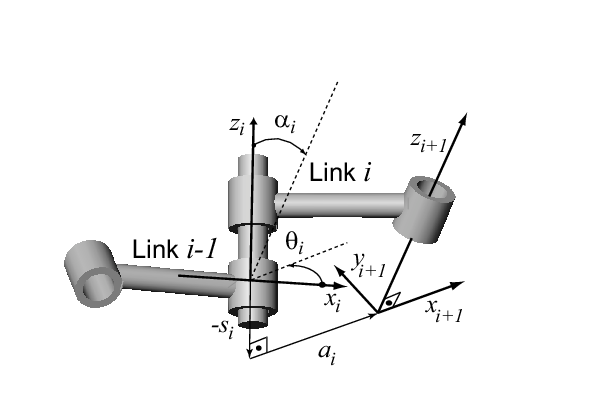
\includegraphics[width=0.75\textwidth]{matriz.png}
    \caption{DH}
    \label{fig:matriz}
\end{figure}

\subsection{Cinemática Diferencial}
La cinemática diferencial tiene como objetivo principal establecer la relación entre las velocidades de las articulaciones de un robot y la velocidad del efector final, o de cualquier otro punto asociado a su estructura. Esta relación se deriva del modelo de cinemática directa y permite obtener información clave sobre el comportamiento del robot, como la detección de singularidades, el análisis de su capacidad de maniobra y la implementación de métodos numéricos para resolver la cinemática inversa de manera iterativa, así como para controlar su movimiento dentro del espacio de trabajo.

A partir del modelo cinemático directo, representado como una función 𝑓(𝑞) que relaciona las coordenadas articulares con la posición del efector, y usando el método de Denavit-Hartenberg con matrices homogéneas, es posible construir una matriz jacobiana. En robótica, esta matriz representa la transformación entre velocidades articulares y velocidades lineales y angulares del efector final. Aunque existen distintos tipos de jacobianas, la más común es la que transforma entre el espacio articular y el espacio cartesiano.

En este modelo no se consideran fuerzas como la inercia o el rozamiento, ya que se analiza el robot como si fuera una masa puntual. Por ello, la cinemática diferencial se centra únicamente en el estudio del movimiento, sin involucrar aspectos dinámicos.

\begin{figure}[H]
    \centering
    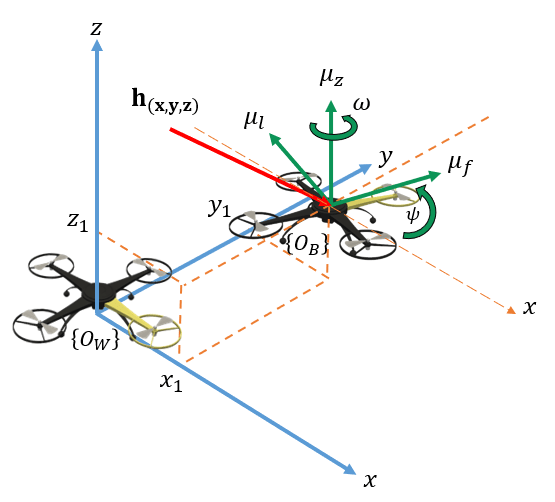
\includegraphics[width=0.50\textwidth]{img/Modelo-cinematico.png}
    \caption{Modelo diferencial}
    \label{fig:Modelo-cinematico}
\end{figure}

\subsection{Cinemática Inversa}
En robótica, la cinemática inversa se encarga de determinar los valores articulares necesarios para que el efector final del robot alcance una posición y orientación específicas. Este proceso es esencial, ya que el control del movimiento se realiza directamente sobre las articulaciones, aunque el objetivo esté en el extremo operativo.

Cuando se desea que el robot transite entre dos posturas, este procedimiento forma parte de la planificación de movimiento, donde la cinemática inversa permite convertir trayectorias deseadas en comandos concretos para los actuadores.

Este enfoque también se aplica fuera de la robótica, como en la animación digital o en simulaciones con cámaras móviles, donde se requiere ajustar articulaciones o trayectorias para lograr movimientos realistas y coherentes.

En resumen, mientras que la cinemática directa calcula la posición del efector a partir de los ángulos articulares, la cinemática inversa realiza el proceso opuesto: determina los valores de las articulaciones necesarios para alcanzar una posición deseada en el espacio.


		
		\section{ROS} \label{sec:ros}
El Sistema Operativo de Robots (ROS, por sus siglas en inglés) es un marco de desarrollo de código abierto que proporciona herramientas, bibliotecas y convenciones para facilitar la creación de software para aplicaciones robóticas. Su objetivo principal es simplificar el diseño, la implementación y la reutilización de código, permitiendo que investigadores, desarrolladores e ingenieros trabajen de manera más eficiente y colaborativa.

ROS no es un sistema operativo en el sentido tradicional, sino una capa de middleware que funciona sobre sistemas como Linux, facilitando la comunicación entre distintos componentes de un robot mediante el uso de tópicos, servicios y acciones. Esto permite que sensores, actuadores, controladores y algoritmos de planificación se integren fácilmente en una arquitectura modular y escalable.

Además de ser una plataforma técnica, ROS representa una comunidad global activa de desarrolladores, investigadores y entusiastas que comparten paquetes, soluciones y mejoras, fomentando la innovación abierta y el avance continuo en el campo de la robótica. ROS es ampliamente utilizado tanto en entornos académicos como industriales y ha sido adoptado para simular, controlar y probar sistemas robóticos complejos en tareas como navegación autónoma, manipulación, percepción y más.

Gracias a herramientas como Gazebo para simulación, Rviz para visualización y su integración con lenguajes como Python y C++, ROS se ha consolidado como una de las plataformas más importantes y versátiles en el desarrollo robótico moderno.
\begin{figure}[h]
	\centering
	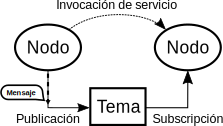
\includegraphics[width=0.5\linewidth]{img/ROS_concepts}
	\caption{Diagrama de comunicación de ROS}
	\label{fig:rosconcepts}
\end{figure}

\subsection{Nodo (Node)}
En ROS (Robot Operating System), un nodo es una unidad básica de ejecución. Se trata de un proceso individual que realiza una tarea específica dentro del sistema robótico. Los nodos pueden encargarse de diversas funciones, como leer datos de sensores, controlar motores, procesar imágenes o ejecutar algoritmos de navegación, entre otros.

Cada nodo en ROS:

Se ejecuta de forma independiente.

Se comunica con otros nodos mediante tópicos, servicios o acciones.

Puede estar programado en lenguajes compatibles con ROS, como Python o C++.

Es modular, lo que permite dividir un sistema complejo en componentes más manejables y reutilizables.

Por ejemplo, en un robot móvil, podría haber un nodo encargado de leer datos del LIDAR, otro que realice el mapeo del entorno, y otro que se encargue de la planificación de trayectorias. Todos estos nodos trabajan en conjunto mediante la infraestructura de comunicación de ROS.

En resumen, un nodo en ROS es un proceso que cumple una función específica dentro de un sistema robótico, facilitando la construcción de arquitecturas distribuidas, escalables y flexibles.

\subsection{Tema (Topic)}
En ROS, un topic representa un canal de comunicación que permite la transmisión de mensajes entre nodos de forma desacoplada y asincrónica. Es uno de los mecanismos fundamentales para el intercambio de información dentro del sistema. Los nodos pueden actuar como publicadores, enviando información a un topic determinado, o como suscriptores, recibiendo información publicada en ese mismo canal. Esto permite que múltiples nodos intercambien información sin necesidad de conocerse entre sí ni mantener una conexión directa.

Este mecanismo es particularmente útil para flujos de datos continuos y en tiempo real, como los que provienen de sensores (cámaras, LIDAR, IMU) o de módulos de control (por ejemplo, el movimiento de un robot móvil). Por ejemplo, un nodo que maneja un sensor LIDAR podría publicar datos en un topic llamado /scan, y un nodo de navegación podría suscribirse a ese topic para usar los datos y generar un mapa del entorno.

El sistema de topics favorece la escalabilidad, ya que múltiples nodos pueden suscribirse al mismo topic sin afectar al publicador. Además, ROS proporciona herramientas como rostopic list, rostopic echo y rqt_graph para monitorear y depurar estas comunicaciones en tiempo real.

\subsection{Mensaje (Message)}
Un mensaje en ROS es una estructura de datos que se transmite entre nodos a través de un topic. Cada mensaje tiene un tipo definido y puede contener campos de datos básicos como enteros, flotantes, booleanos, cadenas de texto, o estructuras más complejas como vectores, posiciones 3D, matrices, etc. Estos mensajes están definidos en archivos .msg, lo que permite mantener una estructura estándar y reutilizable.

Los mensajes garantizan la interoperabilidad entre nodos escritos en diferentes lenguajes de programación (como C++ o Python), ya que ROS maneja la serialización y deserialización automáticamente.

\subsection{Servicio (Service)}
A diferencia de los topics, que están diseñados para comunicaciones unidireccionales y continuas, los servicios en ROS están diseñados para interacciones bidireccionales y sincrónicas, donde se espera una respuesta específica tras una solicitud. Siguen el modelo cliente-servidor, donde un nodo cliente envía una solicitud (request) a un nodo servidor, el cual procesa la solicitud y devuelve una respuesta (response).

Los servicios se definen en archivos .srv, donde se especifican los campos del request y del response, separados por ---. Al igual que con los mensajes, ROS incluye varios servicios predefinidos, y también permite crear servicios personalizados.

Una limitación importante de los servicios es que son bloqueantes: el cliente debe esperar la respuesta antes de continuar con su ejecución, lo cual puede ser una desventaja en aplicaciones que requieren alta velocidad de respuesta o concurrencia.

\subsection{Gazebo}
Gazebo es un potente simulador robótico 3D de código abierto que permite simular entornos físicos complejos y robots en tiempo real con una alta fidelidad física. Gracias a su integración con ROS, es posible simular el comportamiento de robots reales sin necesidad de contar con el hardware físico, lo cual es ideal para desarrollo, prueba y validación de algoritmos de navegación, percepción, planificación de trayectorias y control.

Gazebo puede simular sensores como cámaras RGB y de profundidad, IMUs, LIDARs, GPS, y también puede emular diferentes tipos de terrenos, obstáculos y condiciones ambientales. Utiliza motores de física como ODE (Open Dynamics Engine) o Bullet para calcular interacciones físicas, colisiones, fricción, gravedad, etc.

\subsection{RViz}
RViz (ROS Visualization) es una herramienta gráfica interactiva de ROS que permite visualizar, en un espacio tridimensional, la información que fluye dentro del sistema robótico. Esto incluye visualizaciones del modelo del robot, datos de sensores (como cámaras, LIDAR, mapas), marcos de referencia (tf), trayectorias planificadas, objetivos de navegación, y mucho más.

RViz es fundamental durante el desarrollo de sistemas en ROS porque permite entender cómo el robot “percibe” su entorno y cómo está reaccionando ante diferentes situaciones. Los desarrolladores pueden depurar problemas, validar resultados y ajustar configuraciones directamente desde la interfaz.

La visualización se organiza en "Displays", que son módulos que se pueden añadir o quitar según las necesidades. Por ejemplo, un display de tipo LaserScan puede mostrar la información de un sensor LIDAR, mientras que uno de tipo Path puede mostrar la ruta que el robot planea seguir.

Además, RViz permite la interacción con el sistema, como seleccionar metas de navegación mediante clics o visualizar el resultado de algoritmos de detección de objetos, todo en tiempo real.


		
		\section{Dinámica} \label{sec:dinamica}

En robótica, el estudio de la dinámica es crucial para modelar, simular y controlar el comportamiento de un robot. Permite predecir cómo responderá un robot a ciertas fuerzas, cómo se moverán sus partes articuladas y cómo mantener la estabilidad al realizar tareas complejas.

La dinámica robótica considera:

Modelos dinámicos del robot (incluyendo masa, centros de masa, inercia, par de motores, fricción).

Ecuaciones de movimiento basadas en la formulación de Euler-Lagrange o la formulación de Newton-Euler, que describen cómo las fuerzas y momentos aplicados generan aceleraciones y movimientos.

Control de movimiento dinámico, como el control de par, el control por impedancia/admitancia, o el control dinámico inverso, que permite movimientos suaves, seguros y adaptativos.

Estas ecuaciones permiten diseñar controladores robustos, como los utilizados en brazos robóticos industriales, exoesqueletos, robots bípedos o manipuladores móviles.


\subsection{Matriz de masa o inercia}

En el estudio de la dinámica robótica, la matriz de masa o inercia, denotada como $\mathbf{M}(q)$, representa cómo la masa y su distribución afectan el movimiento de un sistema robótico en función de su configuración articular $q$. Esta matriz es una parte esencial del modelo dinámico del robot y aparece en la ecuación general del movimiento:

\[
\mathbf{M}(q)\ddot{q} + \mathbf{C}(q, \dot{q})\dot{q} + \mathbf{G}(q) = \boldsymbol{\tau}
\]

donde $\ddot{q}$ representa las aceleraciones articulares, $\dot{q}$ las velocidades, $\mathbf{C}$ los efectos centrífugos y de Coriolis, $\mathbf{G}$ las fuerzas de gravedad, y $\boldsymbol{\tau}$ los torques aplicados por los actuadores.

Bajo la simplificación de ausencia de fuerzas externas, la aceleración máxima alcanzable por una articulación está dada por:

\[
\ddot{q}_{\text{máx}} = \mathbf{M}^{-1}(q) \boldsymbol{\tau}_{\text{máx}}
\]

Esto implica que la aceleración que puede alcanzar el robot está directamente determinada por la inversa de la matriz de inercia y el torque máximo disponible. Una mayor inercia (masa concentrada o distribución desfavorable) reducirá la aceleración que puede generarse con un mismo torque. Además, debido al acoplamiento dinámico entre articulaciones, la matriz de inercia puede contener términos no diagonales que indican cómo el movimiento de una articulación influye en otras.

Comprender y modelar correctamente la matriz de inercia es fundamental para el diseño de controladores dinámicos, simulaciones físicas realistas y sistemas robóticos seguros y eficientes.


\subsection{Matriz de coriolis}

La matriz de Coriolis, representada como $\mathbf{C}(q, \dot{q})$, forma parte del modelo dinámico de un robot y está asociada a los efectos centrífugos y de Coriolis que aparecen cuando el sistema está en movimiento. Esta matriz aparece en la ecuación dinámica general:

\[
\mathbf{M}(q)\ddot{q} + \mathbf{C}(q, \dot{q})\dot{q} + \mathbf{G}(q) = \boldsymbol{\tau}
\]

donde $\mathbf{M}(q)$ es la matriz de inercia, $\ddot{q}$ y $\dot{q}$ son la aceleración y velocidad articulares, $\mathbf{G}(q)$ representa los efectos gravitacionales, y $\boldsymbol{\tau}$ es el vector de torques actuadores.

La matriz $\mathbf{C}(q, \dot{q})$ modela las **fuerzas y torques no lineales** que surgen debido al movimiento conjunto de varias articulaciones. Estas fuerzas incluyen:
\begin{itemize}
	\item \textbf{Fuerzas centrífugas}, que aparecen en sistemas giratorios incluso si las velocidades angulares son constantes.
	\item \textbf{Fuerzas de Coriolis}, que dependen de la interacción entre velocidades articulares, típicamente representadas como términos bilineales en $\dot{q}$.
\end{itemize}

La matriz de Coriolis no es única, pero debe cumplir con ciertas propiedades para garantizar la estabilidad del sistema, como que la matriz $\dot{\mathbf{M}}(q) - 2\mathbf{C}(q, \dot{q})$ sea antisimétrica.

Computacionalmente, los elementos de $\mathbf{C}(q, \dot{q})$ pueden calcularse a partir de los coeficientes de Christoffel derivados de la matriz de inercia:

\[
C_{ijk} = \frac{1}{2} \left( \frac{\partial M_{ij}}{\partial q_k} + \frac{\partial M_{ik}}{\partial q_j} - \frac{\partial M_{jk}}{\partial q_i} \right)
\]

y luego combinados con las velocidades:

\[
C_{ij} = \sum_{k=1}^{n} C_{ijk} \dot{q}_k
\]

La inclusión de esta matriz en simulaciones y controladores permite compensar correctamente los efectos dinámicos en robots en movimiento, mejorando la precisión del control, especialmente a altas velocidades o en sistemas con brazos largos o cargas pesadas. Es un componente fundamental en técnicas de control dinámico inverso y control robusto.



\subsection{Vector de gravedad}

Cuando el robot está extendido horizontalmente, el vector de gravedad tiene su mayor efecto sobre el sistema debido al momento que genera respecto al eje de rotación de cada articulación. En esta posición, el centro de masa del brazo robótico (o del sistema en general) está más alejado del eje base, lo que incrementa el \textbf{momento de torsión (torque)} requerido para mantener la posición o mover el brazo.

El \textbf{momento generado por la gravedad} se calcula como:

\begin{equation}
	\tau = r \times F_g = r \cdot m \cdot g \cdot \sin(\theta)
\end{equation}

Donde:
\begin{itemize}
	\item $\tau$ es el torque debido al peso,
	\item $r$ es la distancia desde el eje de rotación al centro de masa,
	\item $m$ es la masa del segmento,
	\item $g$ es la aceleración gravitacional,
	\item $\theta$ es el ángulo entre el brazo y la dirección vertical (siendo $90^\circ$ cuando está horizontal).
\end{itemize}

Cuando el brazo está completamente horizontal ($\theta = 90^\circ$), se cumple que $\sin(\theta) = 1$, y por lo tanto el torque alcanza su valor máximo:

\begin{equation}
	\tau_{\text{máx}} = r \cdot m \cdot g
\end{equation}

Este torque debe ser completamente contrarrestado por la fuerza generada por los motores, ya que, de lo contrario, el brazo caerá bajo el efecto de la gravedad. Si los motores no generan suficiente torque, no podrán sostener o mover el brazo en esta posición. Por eso, es fundamental dimensionar correctamente los motores considerando este escenario crítico.


\subsection{Fricción}

La \textbf{fricción} es una fuerza que se opone al movimiento relativo entre dos superficies en contacto. Es una fuerza de resistencia que actúa en dirección contraria al desplazamiento o intento de desplazamiento de un objeto.

\subsection{Tipos de fricción}
\begin{itemize}
	\item \textbf{Fricción estática:} Se presenta cuando un objeto está en reposo, y es la fuerza que debe superarse para que comience a moverse. Generalmente, es mayor que la fricción cinética.
	
	\item \textbf{Fricción cinética (o dinámica):} Ocurre cuando el objeto ya está en movimiento. Esta fricción sigue actuando en contra del movimiento y su valor es constante y menor que el de la fricción estática.
	
	\item \textbf{Fricción por rodadura:} Se da cuando un objeto rueda sobre una superficie, como una llanta o un rodillo. Suele ser mucho menor que la fricción por deslizamiento.
\end{itemize}

\subsection{Factores que afectan la fricción}
\begin{itemize}
	\item La naturaleza de las superficies (rugosidad o tipo de material).
	\item La fuerza normal (la fuerza perpendicular entre las superficies en contacto).
\end{itemize}

Cabe mencionar que, en condiciones ideales, la fricción no depende del área de contacto ni de la velocidad de movimiento.

\subsection{Fórmula general de la fricción}
La fuerza de fricción se puede calcular mediante la siguiente expresión:

\begin{equation}
	f = \mu \cdot N
\end{equation}

Donde:
\begin{itemize}
	\item $f$ es la fuerza de fricción,
	\item $\mu$ es el coeficiente de fricción (depende de los materiales en contacto),
	\item $N$ es la fuerza normal (perpendicular a la superficie).
\end{itemize}

\subsection{Perturbaciones}

Una \textbf{perturbación} es cualquier influencia externa que altera el comportamiento normal o esperado de un sistema. En términos generales, se trata de una desviación o interferencia que afecta el funcionamiento, la estabilidad o el rendimiento del sistema, ya sea de forma temporal o permanente.

Estas pueden ser causadas por factores como cambios en el entorno, errores de medición, vibraciones, variaciones en la carga o cualquier otra condición no prevista que afecte la operación normal del sistema.

Aunque en esta sección no se profundiza en su análisis, es importante reconocer que las perturbaciones son inevitables en sistemas reales, y deben ser consideradas en el diseño y control de sistemas automáticos o robóticos.

		
		\section{Control}
En la Figura~\ref{fig:diagrama-de-robot-industrial}. se muestra el diagrama de bloques correspondiente al sistema de control de un robot industrial. Este diagrama describe el flujo de información desde la entrada del usuario hasta el movimiento del robot, incluyendo el control, la planificación de trayectoria y el modelo dinámico.

\begin{itemize}
	\item \textbf{Valores definidos por el usuario:} Se introducen parámetros como puntos coordenados, velocidad mínima, aceleración mínima y tipo de trayectoria. Estos definen el objetivo deseado para el efector final del robot.
	
	\item \textbf{Planificación de trayectoria:} Genera valores deseados para el efector final (posición, velocidad, aceleración) en el espacio cartesiano. Estos valores permiten un movimiento suave y seguro del robot.
	
	\item \textbf{Cinemática inversa:} Convierte los valores del efector final a coordenadas articulares (posición $q$, velocidad $\dot{q}$ y aceleración $\ddot{q}$), ya que el robot opera en este espacio.
	
	\item \textbf{Controlador:} Calcula el error entre la trayectoria deseada ($Z_d$) y la trayectoria real ($\hat{Z}$), y genera las señales de control necesarias (fuerza lineal o torque rotacional) para corregirlo.
	
	\item \textbf{Dinámica del robot:} Representa el modelo físico del robot, que puede ser no lineal ($\dot{x} = f(x, u)$) o

 \autoref{fig:diagrama-de-robot-industrial}.

\begin{figure}[h]
	\centering
	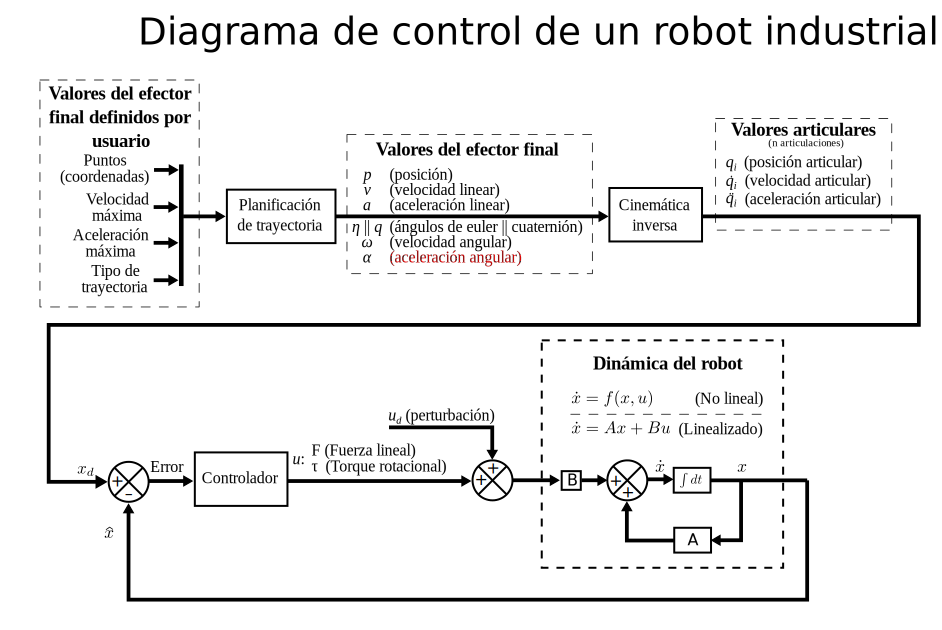
\includegraphics[width=\linewidth]{img/Diagrama_robot_industrial}
	\caption{Diagrama de bloques de un robot industrial}
	\label{fig:diagrama-de-robot-industrial}
\end{figure}

	
	% Capítulo 3: Desarrollo
	\chapter{Introducción} \label{chap:introduccion}

El presente trabajo tiene como objetivo documentar y analizar el desarrollo de un proyecto robótico realizado durante el semestre, el cual integra los principales conceptos estudiados en la asignatura de Robótica. Para este proyecto, se seleccionó un modelo de robot descargado directamente desde una plataforma en línea, el cual ya contaba con un diseño de ensamblado estructural completo. Esta elección permitió enfocar el trabajo en el análisis cinemático y en la aplicación de modelos matemáticos y conceptuales clave.

Una vez definido el modelo, se procedió a identificar sus ejes de rotación y sus coordenadas espaciales, lo que permitió establecer los parámetros necesarios para construir las tablas de Denavit-Hartenberg. A partir de estas tablas, se desarrolló la cinemática directa del robot, permitiendo determinar la posición y orientación del efector final en función de las variables articulares. Posteriormente, se abordó la cinemática diferencial, lo cual facilitó el análisis de velocidades y permitió una mejor comprensión del comportamiento dinámico del sistema.

Además, se resolvió el problema de la cinemática inversa, fundamental para el control del robot en tareas específicas, ya que permite calcular los valores articulares necesarios para alcanzar una determinada posición en el espacio. Todos estos análisis y cálculos se realizaron en concordancia con los contenidos abordados a lo largo del semestre, consolidando así los conocimientos teóricos mediante su aplicación práctica.

Este informe detalla cada una de estas etapas, presentando los fundamentos teóricos, los métodos aplicados y los resultados obtenidos, con el fin de demostrar el dominio adquirido en el manejo de herramientas y conceptos fundamentales en el campo de la robótica.
	
		\section{Características del Robot} \label{sec:caracteristicas_del_robot}

El primer paso consistió en analizar la estructura del robot y definir su configuración geométrica mediante la \textbf{tabla de Denavit-Hartenberg (DH)}. Este paso fue fundamental, ya que permitió establecer los parámetros necesarios para describir la posición y orientación relativa entre los eslabones del robot.

\begin{table}[H]
	\centering
	\caption{Parámetros Denavit-Hartenberg del robot KUKA KR-16}
	\label{tab:dh_kuka}
	\begin{tabular}{c|c|c|c|c|c|c|c|c}
		\toprule
		$i$ & $\theta$ ($^\circ$) & $d$ (mm) & $a$ (mm) & $\alpha$ ($^\circ$) & Tipo & $\theta_{min}$ ($^\circ$) & $\theta_{max}$ ($^\circ$) & Velocidad ($^\circ$/s) \\
		\midrule
		1 & 0    & 675  & 260  & -90  & r & -185 & 185  & 156 \\
		2 & 0    & 680  & 0    & -155 & r & -155 & 35   & 156 \\
		3 & -90  & 0    & 0    & -90  & r & -130 & 154  & 156 \\
		4 & 0    & -670 & 0    & -90  & r & -350 & 350  & 330 \\
		5 & 0    & 0    & 0    & -90  & r & -130 & 130  & 330 \\
		6 & 0    & -158 & 180  & -350 & r & -350 & 350  & 615 \\
		\bottomrule
	\end{tabular}
\end{table}


\bigskip
\noindent
\textbf{Donde:}
\begin{description}
	\item[N] Número de la articulación.
	\item[\(\theta\)] Ángulo articular (grados).
	\item[\(d\)] Desplazamiento a lo largo del eje \(z\) (milímetros).
	\item[\(a\)] Longitud del eslabón (milímetros).
	\item[\(\alpha\)] Ángulo entre ejes \(z\) consecutivos (grados).
	\item[Tipo] ‘r’ para articulación rotacional.
	\item[\(q_{\min}\), \(q_{\max}\)] Límites de posición (grados).

\end{description}



		
			\subsection{Partes} \label{subsec:partes}
\subsection*{Componentes principales del robot KUKA KR 16}

El robot KUKA KR 16 es un manipulador industrial de seis grados de libertad. A continuación, se describen brevemente sus principales componentes:

\begin{itemize}
	\item \textbf{Base (Eje 1):} Es la estructura fija sobre la que se monta el robot. Contiene el motor del primer eje, permitiendo rotación horizontal del brazo completo.
	
	\item \textbf{Eje 2 (Brazo inferior):} Conecta la base con el brazo superior. Este eje permite un movimiento similar al de un codo, desplazando el brazo hacia adelante y hacia atrás.
	
	\item \textbf{Eje 3 (Brazo superior):} Proporciona movimiento vertical adicional, incrementando el alcance en altura.
	
	\item \textbf{Eje 4 (Muñeca rotacional):} Permite la rotación del extremo del brazo sobre su propio eje, facilitando la orientación de la herramienta.
	
	\item \textbf{Eje 5 (Muñeca de inclinación):} Controla la inclinación hacia arriba o abajo del efector final, aportando mayor precisión de orientación.
	
	\item \textbf{Eje 6 (Muñeca de rotación final):} Permite una rotación axial adicional del efector final, crucial para tareas como ensamblado o soldadura.
	
	\item \textbf{Brida de montaje (flange):} Es la interfaz mecánica donde se monta la herramienta o efector final (pinzas, sensores, etc.).
	
	\item \textbf{Cables y conexiones:} Incluye tanto cableado interno como externo para transmisión de señales y potencia entre los actuadores, sensores y el controlador.
	
	\item \textbf{Controlador KR C4:} Es la unidad de procesamiento y control del robot. Ejecuta programas, regula el movimiento de los motores y gestiona entradas/salidas.
	
\end{itemize}

\textbf{Especificaciones técnicas destacadas:}
\begin{itemize}
	\item Grados de libertad: 6 (todos rotacionales).
	\item Alcance máximo: 1612 mm.
	\item Carga útil nominal: 16 kg.
	\item Repetibilidad: $\pm$0.04 mm.
	\item Montaje: suelo, techo o pared.
	\item Protección: IP65 para el cuerpo del robot e IP65 para la muñeca.
\end{itemize}

\subsubsection{Motores} \label{subsubsec:motores}
	\begin{itemize}
		\item \textbf{Motor utilizado:} Servomotor SG90 (referencia a la hoja de datos del fabricante: TowerPro SG90).
		
		\item \textbf{Características principales:}
		\begin{itemize}
			\item \textbf{Masa:} 9 gramos.
			\item \textbf{Torque máximo:} 2.5 kg·cm (aproximadamente 0.245 Nm).
			\item \textbf{Velocidad máxima:} 0.1 s/60° a 4.8V.
			\item \textbf{Voltaje de operación:} 4.8V – 6V.
		\end{itemize}
		
		\item \textbf{Transmisiones y reductores:}
		\begin{itemize}
			\item Los motores están acoplados a engranajes internos tipo corona para reducir velocidad y aumentar torque.
			\item Las pinzas cuentan con una transmisión mecánica simple de tipo tornillo sin fin.
			\item \textbf{Razón de reducción estimada:} 10:1.
		\end{itemize}
		
		\item \textbf{Distribución de los motores en el robot:}
		\begin{itemize}
			\item \textbf{Motor 1:} Base del robot – permite giro horizontal.
			\item \textbf{Motor 2:} Articulación del brazo – controla elevación y descenso.
			\item \textbf{Motor 3:} Pinza – apertura y cierre mediante engranaje y reductor.
		\end{itemize}
		
	\end{itemize}
	
\end{frame}

\subsubsection{Eslabones} \label{subsubsec:eslabones}
	
	\textbf{Características físicas de los eslabones:}
	
	\begin{table}[ht]
		\centering
		\begin{tabular}{|c|c|c|c|c|}
			\hline
			\textbf{Eslabón} & \textbf{Masa (g)} & \textbf{Longitud (cm)} & \textbf{Material} & \textbf{Inercia (g·cm\textsuperscript{2})} \\
			\hline
			1 & 50 & 10 & PLA (impresión 3D) & 42.0 \\
			2 & 65 & 12 & PLA (impresión 3D) & 58.5 \\
			3 & 40 & 8  & PLA (impresión 3D) & 26.0 \\
			\hline
		\end{tabular}
		\caption{Parámetros físicos de cada eslabón del robot}
	\end{table}
	
	\vspace{0.3cm}
	\textbf{Nota:} La inercia fue estimada considerando cuerpos cilíndricos y distribución uniforme de masa.
	
\end{frame}

			
			\subsection{Límites y propiedades dinámicas de las articulaciones} \label{subsec:limites_propiedades}

En los parametros del robot se presentan los parámetros Denavit-Hartenberg (DH) utilizados para modelar el robot KUKA KR-16. A partir de la columna \texttt{tipo}, se especifica que todas las articulaciones del robot son de tipo \textbf{rotacional (R)}, ya que se trata de un robot articulado de 6 grados de libertad. Esto implica que cada articulación permite una rotación alrededor de un eje fijo, lo que es característico de este tipo de manipuladores.

Las columnas $\theta_{\text{min}}$ y $\theta_{\text{max}}$ representan los \textbf{límites angulares} de cada articulación. Estos valores son esenciales para restringir el movimiento del robot dentro de un rango físico seguro y evitar configuraciones que puedan ser inalcanzables o peligrosas.

La columna \texttt{Velocidad del eje} muestra la \textbf{velocidad máxima} en grados por segundo que puede alcanzar cada articulación. Esta información es importante tanto para el diseño de trayectorias como para la simulación del desempeño del robot en tiempo real.

%\subsection{Modelo dinámico del robot}
%\textit{Esta sección ha sido comentada debido a que el modelo dinámico del robot no fue completado durante el desarrollo del proyecto. Se propone incluirla como trabajo futuro para continuar con el análisis de fuerzas y torques necesarios para el control del manipulador.}

		
		\section{Proceso de Cinemática} \label{sec:proceso_cinematica}

En esta sección se describe el proceso para calcular las diferentes etapas de la cinemática del robot desarrollado, el cual fue descargado inicialmente de internet y adaptado para nuestro uso. Todo el código está disponible en el repositorio de GitHub, por lo que aquí se presentarán solo las partes más relevantes para la comprensión del trabajo.

\subsection{Cinemática Directa}

La cinemática directa se encarga de obtener la posición y orientación del efector final del robot dada una configuración específica de sus articulaciones.

Una parte fundamental del código consiste en crear la matriz homogénea de referencia inicial, que representa la orientación y posición del efector al inicio del movimiento. Para ello, se utiliza la función \texttt{euler2rotMat} que convierte ángulos de Euler a una matriz de rotación:

\begin{matlabcode}{matlab}
	R_inicial = euler2rotMat(orientacion_inicial, secuencia);
	Matriz_cero = [0 0 0];
	A0 = [R_inicial posicion_inicial;
	Matriz_cero 1];
\end{matlabcode}

Aquí, \texttt{A0} representa la matriz homogénea inicial, donde \texttt{posicion_inicial} es un vector con la posición en el espacio y \texttt{R_inicial} la orientación asociada.

Posteriormente, se leen los parámetros de Denavit-Hartenberg desde un archivo CSV para configurar el robot y sus límites de movimiento:

\begin{matlabcode}{matlab}
	dh = readtable('datos\tabla_DH\robotFinal.csv');
	robot = crear_robot(dh, A0);
\end{matlabcode}

Con el robot definido, se genera una trayectoria periódica para las articulaciones, con un período de 2 segundos:

\begin{matlabcode}{matlab}
	periodo = 2;    % Periodo del movimiento cíclico
	[q, dq, ddq] = trayectoria_q(robot, t, periodo);
\end{matlabcode}

Esto permite que las articulaciones realicen un movimiento repetitivo, facilitando el análisis del comportamiento dinámico y la validación de la cinemática.

Los resultados y gráficos relacionados se pueden consultar en el capítulo \autoref{chap:resultados}.

\subsection{Cinemática Diferencial}

La cinemática diferencial permite relacionar las velocidades articulares con la velocidad lineal y angular del efector final. En el código, se calcula el Jacobiano del robot para determinar estas relaciones.

Una parte clave del código es la función que calcula el Jacobiano y lo usa para obtener las velocidades del efector a partir de las velocidades articulares:

\begin{matlabcode}{matlab}
	J = calcular_jacobiano(robot, q);
	v_efector = J * dq;
\end{matlabcode}

Esto es fundamental para control y seguimiento de trayectoria, así como para análisis de singularidades y manipulabilidad.

Los detalles de implementación y resultados gráficos se encuentran en el capítulo \autoref{chap:resultados}.

\subsection{Cinemática Inversa}

Para la cinemática inversa, se busca calcular los valores de las articulaciones que lleven al efector a una posición y orientación deseadas. El método implementado utiliza un algoritmo iterativo con control de convergencia.

La función principal recibe como entradas el robot, la posición deseada, la tolerancia, el máximo número de iteraciones, el parámetro de ajuste y el número de muestras:

\begin{matlabcode}{matlab}
	function [q_sol, p_sol] = cinematica_inv(r, p_des, tol, max_iter, alpha, numMuestras)
\end{matlabcode}

Este algoritmo itera ajustando las articulaciones hasta que la posición obtenida esté dentro de la tolerancia requerida o se alcance el número máximo de iteraciones.

Los resultados de este procedimiento, así como las gráficas de convergencia y trayectorias, están documentados en el capítulo \autoref{chap:resultados}.

		
		\section{Control}
En la Figura~\ref{fig:diagrama-de-robot-industrial}. se muestra el diagrama de bloques correspondiente al sistema de control de un robot industrial. Este diagrama describe el flujo de información desde la entrada del usuario hasta el movimiento del robot, incluyendo el control, la planificación de trayectoria y el modelo dinámico.

\begin{itemize}
	\item \textbf{Valores definidos por el usuario:} Se introducen parámetros como puntos coordenados, velocidad mínima, aceleración mínima y tipo de trayectoria. Estos definen el objetivo deseado para el efector final del robot.
	
	\item \textbf{Planificación de trayectoria:} Genera valores deseados para el efector final (posición, velocidad, aceleración) en el espacio cartesiano. Estos valores permiten un movimiento suave y seguro del robot.
	
	\item \textbf{Cinemática inversa:} Convierte los valores del efector final a coordenadas articulares (posición $q$, velocidad $\dot{q}$ y aceleración $\ddot{q}$), ya que el robot opera en este espacio.
	
	\item \textbf{Controlador:} Calcula el error entre la trayectoria deseada ($Z_d$) y la trayectoria real ($\hat{Z}$), y genera las señales de control necesarias (fuerza lineal o torque rotacional) para corregirlo.
	
	\item \textbf{Dinámica del robot:} Representa el modelo físico del robot, que puede ser no lineal ($\dot{x} = f(x, u)$) o

 \autoref{fig:diagrama-de-robot-industrial}.

\begin{figure}[h]
	\centering
	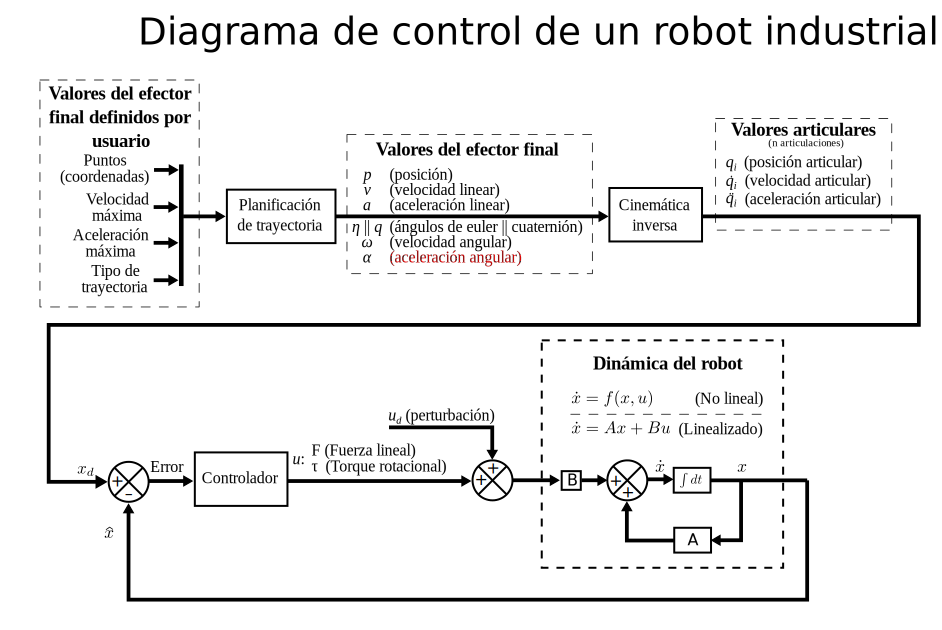
\includegraphics[width=\linewidth]{img/Diagrama_robot_industrial}
	\caption{Diagrama de bloques de un robot industrial}
	\label{fig:diagrama-de-robot-industrial}
\end{figure}

		
		\input{capitulos/Desarrollo/Simulación}
	
	% Capítulo 4: Resultados
	\chapter{Resultados} \label{chap:resultados}
En este capítulo se presentan los resultados obtenidos durante la implementación y simulación del robot. Se muestran las salidas de la cinemática directa e inversa, las gráficas que describen el comportamiento de las articulaciones, y la validación de la simulación en entorno virtual.
\begin{figure}
	\centering
	\includegraphics[width=0.65\linewidth]{../501289512_1030174882084249_9101665985105919383_n}
	\caption{}
	\label{fig:50128951210301748820842499101665985105919383n}
\end{figure}



\section{Cinemática Directa}

La cinemática directa permite obtener la posición y orientación del efector final a partir de los ángulos articulares. 

A continuación se presentan las configuraciones espaciales calculadas para diferentes posiciones articulares, demostrando la precisión del modelo y su correcta implementación.


\begin{figure}
	\centering
	\includegraphics[width=0.65\linewidth]{../494824317_1444026277012878_2465681822553122772_n}
	\caption{}
	\label{fig:49482431714440262770128782465681822553122772n}
\end{figure}

Los resultados muestran que el robot alcanza las posiciones esperadas conforme a la trayectoria generada, validando el modelo DH y la matriz homogénea inicial utilizada.

\section{Cinemática Inversa}

La cinemática inversa permite determinar los ángulos articulares que debe adoptar el robot para alcanzar una posición y orientación deseada del efector final. 

En este proyecto, se implementó una función iterativa que ajusta los valores de las articulaciones hasta alcanzar la posición objetivo con una tolerancia definida. Esta función utiliza un modelo basado en el Jacobiano y se detiene cuando se alcanza la tolerancia o el número máximo de iteraciones.

A continuación, se muestra una gráfica de la trayectoria deseada frente a la trayectoria real obtenida a través de la solución de la cinemática inversa:

\begin{figure}
	\centering
	\includegraphics[width=0.65\linewidth]{../494822215_569383659201449_4831555420233948294_n}
	\caption{}
	\label{fig:4948222155693836592014494831555420233948294n}
\end{figure}



\section{Cinemática Diferencial}

La cinemática diferencial relaciona las velocidades articulares con la velocidad del efector final, siendo fundamental para el control y la planificación dinámica.

En la siguiente gráfica se presenta la evolución de las velocidades lineales y angulares del efector durante el movimiento cíclico de las articulaciones.

\begin{figure}
	\centering
	\includegraphics[width=0.65\linewidth]{../494860605_1270406011321680_2515407621569777704_n}
	\caption{}
	\label{fig:49486060512704060113216802515407621569777704n}
\end{figure}



Los datos confirman que la velocidad del efector responde adecuadamente a los cambios en las velocidades articulares, lo que es esencial para el seguimiento de trayectorias suaves.

\section{Gráficas de las Articulaciones}

Se muestran las gráficas de las posiciones angulares de las articulaciones a lo largo del tiempo, junto con sus velocidades y aceleraciones, obtenidas mediante la trayectoria programada.

\begin{figure}
	\centering
	\includegraphics[width=0.65\linewidth]{../494820732_1414021652877929_4111381788106881331_n}
	\caption{}
	\label{fig:49482073214140216528779294111381788106881331n}
\end{figure}


Las gráficas reflejan el movimiento cíclico con un periodo de 2 segundos, confirmando la correcta generación y ejecución de la trayectoria.

\section{Simulación}

Finalmente, se validó el comportamiento del robot mediante simulación en entorno virtual, utilizando herramientas como \textit{Gazebo}, \textit{RViz} y \textit{MoveIt!}.

\begin{figure}
	\centering
	\includegraphics[width=0.65\linewidth]{../494817014_1795811371279923_6575303978208375908_n}
	\caption{}
	\label{fig:49481701417958113712799236575303978208375908n}
\end{figure}

\begin{figure}
	\centering
	\includegraphics[width=0.65\linewidth]{../494823569_1884423959049659_5086006415803663602_n}
	\caption{}
	\label{fig:49482356918844239590496595086006415803663602n}
\end{figure}

\begin{figure}
	\centering
	\includegraphics[width=0.7\linewidth]{../502117343_1786009252327352_787892156864766060_n}
	\caption{}
	\label{fig:5021173431786009252327352787892156864766060n}
\end{figure}


La simulación confirma la coordinación entre las articulaciones y la correcta ejecución de la cinemática programada, incluyendo el movimiento simultáneo de las dos pinzas.

Además, se exploró la integración de actuadores adicionales como el electroimán, lo cual se encuentra en etapa experimental.

	
	% Capítulo 5: Conclusiones
	\chapter{Conclusiones} \label{sec:conclusiones}
	\section{Arvizu Michelle}
Durante el desarrollo de este proyecto, enfrenté varios retos que, aunque frustrantes en su momento, terminaron siendo grandes oportunidades de aprendizaje. Uno de los principales problemas fue entender y aplicar correctamente los conceptos de cinemática inversa. Al principio, me costó mucho lograr que el algoritmo convergiera a una solución estable; algunas veces el robot no alcanzaba la posición deseada o se movía de forma errática. Me tomó tiempo entender cómo ajustar los parámetros del algoritmo, como la tolerancia y el paso, y cómo evitar errores por cercanía a singularidades.

Otro problema que tuve fue con la simulación en Ubuntu. No tenía experiencia previa con herramientas como Gazebo, RViz o MoveIt, y tampoco con el uso de una máquina virtual. Instalar todo correctamente, hacer que el robot se visualizara y que respondiera a los comandos fue un proceso largo, con muchos errores de dependencia y configuración. Pero gracias al tutorial, a la documentación del repositorio y a la ayuda del equipo, logré completar la simulación y ver el robot moverse con sus dos pinzas coordinadas, lo cual me dio mucha satisfacción.
	\section{Carranza Jesús}
Lo que más aprendí fue a no rendirme cuando las cosas no salen a la primera. A veces pasaba horas intentando que algo funcionara y parecía imposible, pero con paciencia y pruebas fui entendiendo cómo se conectaban las piezas. También aprendí mucho sobre trabajo en equipo, comunicación y organización del código. Aunque al principio descargamos el modelo del robot desde internet, adaptarlo a nuestro proyecto y entenderlo por dentro fue clave para poder modificarlo y lograr que funcionara con nuestras propias trayectorias y simulaciones.

Este proyecto me ayudó a afianzar mis conocimientos en robótica y me motivó a seguir explorando áreas como control, automatización y simulación, que antes me parecían demasiado complicadas. Ahora me siento más preparado para enfrentar proyectos más grandes y con más confianza para resolver problemas técnicos.


	\section{Montoya Morelia}
Me enfoqué principalmente en la parte de control, aunque al principio no entendía muy bien cómo aplicarlo en este contexto. Fue difícil interpretar cómo el Jacobiano influye en la estabilidad del robot y cómo se puede usar para diseñar leyes de control. No logramos implementar un control avanzado como queríamos, pero el simple hecho de entender cómo se conectan las velocidades articulares con la posición del efector fue muy valioso para mí.

Además, fue la primera vez que trabajé con ROS y todas las herramientas que conlleva: instalar Gazebo, configurar URDF, y hacer que todo corriera en WSL fue bastante abrumador. A pesar de eso, ahora me siento mucho más cómodo con estas herramientas y sé que podré usarlas con más soltura en futuros proyectos. Lo más importante que me llevo es que la robótica no es solo matemática y código: también es prueba, error, intuición y trabajo en equipo.


	\section{Moreno Ana}
Participar en este proyecto me sacó completamente de mi zona de confort. Yo tenía más experiencia en diseño mecánico que en programación, así que cuando llegó el momento de usar MATLAB para desarrollar la cinemática, me sentí algo perdida. Pero con ayuda del equipo y revisando el código descargado del repositorio, fui entendiendo cada parte y aprendí mucho sobre cómo se implementan los modelos matemáticos de un robot.

Me gustó especialmente ver cómo la teoría que estudiamos en clase tomaba forma en algo visual y tangible, como ver el robot moverse en Gazebo o probar diferentes trayectorias. Otro aspecto que disfruté fue trabajar con los sensores simulados y pensar en cómo los incorporaríamos en un caso real. Este proyecto me dejó con muchas ganas de seguir aprendiendo sobre integración de sistemas y simulación robótica, y me demostró que incluso cuando las cosas no salen como uno quiere, siempre se aprende algo nuevo.
		
	\titleformat{\chapter}
	{\bfseries\huge}
	{}
	{0pt}
	{~\raisebox{-1.5pt}{}
		\\\vspace{.05cm}\titlerule\\\filcenter #1 \\\vspace{.25cm}\titlerule}
	%{\titlerule\\\vspace{.25cm}\filcenter #1 \\\vspace{.25cm}\titlerule}
	\bibliographystyle{IEEEtranN}
	\newpage\label{bibliografia}
	\addcontentsline{toc}{chapter}{Bibliografía}
	
	% Pulsa Ctrl + Clic Izquierdo en bibliografia para entrar.
	\bibliography{bibliografia}
\end{document}


